\documentclass[a4paper,11pt]{article}
\usepackage[T1]{fontenc}
\usepackage[utf8]{inputenc}
\usepackage{lmodern}
\usepackage[top=2cm, bottom=2cm, left=2cm, right=2cm]{geometry}
\usepackage{graphicx}
\usepackage{listings}
\usepackage{color}

\title{Implementation of a compiler for an imperative language\\IMP}
\author{Remy Detobel \& Denis Hoornaert}
 
\definecolor{codegreen}{rgb}{0,0.6,0}
\definecolor{codegray}{rgb}{0.5,0.5,0.5}
\definecolor{codepurple}{rgb}{0.58,0,0.82}
\definecolor{backcolour}{rgb}{0.95,0.95,0.92}
 
\lstdefinestyle{mystyle}{
    backgroundcolor=\color{backcolour},   
    commentstyle=\color{codegreen},
    keywordstyle=\color{magenta},
    numberstyle=\tiny\color{codegray},
    stringstyle=\color{codepurple},
    basicstyle=\footnotesize,
    breakatwhitespace=false,         
    breaklines=true,                 
    captionpos=b,                    
    keepspaces=true,                 
    numbers=left,                    
    numbersep=5pt,                  
    showspaces=false,                
    showstringspaces=false,
    showtabs=false,                  
    tabsize=2
}
 
\lstset{style=mystyle}

\begin{document}

\maketitle

\section{Introduction}

  The project aim is to implement a compiler for a 'simple' imperative language named \textit{IMP}. Like any imperative programming language, \textit{IMP} is structured of mainstream features such as \textit{keywords} (\verb|if|, \verb|while|, ... statements), the use of \textit{variables}, the use \textit{numbers} and the use of \textit{comments}.
  The form of these features follows some defined rules~:
  \begin{itemize}
    \item a \textit{variable} is a sequence of alphanumeric characters that must start by a letter.
    \item a \textit{number} is a sequence of one or more digits.
    \item a \textit{comment} must start by the combination \verb|(*| and ends by the reversed combination \verb|*)|.
  \end{itemize}
  The compilation scheme is generally divided in three main phases~: analysis, synthesis and optimization. The phases are themselves composes of different steps. For instance, the analysis phase is composed of \textit{lexical analysing} step (or \textit{scanning}), a \textit{syntax analysing} step (or \textit{parsing}) and a \textit{semantic analysing} step. In this assignment, the focus is set on the \textit{analysis phase}.
  % Replace it by a proper figure.
  \begin{center}
    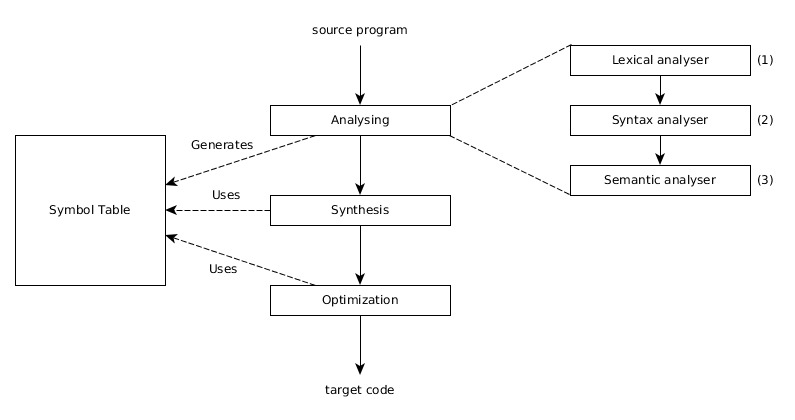
\includegraphics[scale=0.5]{./img/phase_of_compiler.jpg}\\
    \textit{Figure 1~-~Compilation phases.}
  \end{center}
  
\section{Implementation of the lexical analyser}

  In the so called "Dragon book"\footnote{V. Aho, A., 2007. \textit{Compilers~: Principles, techniques, \& Tools.} 2nd ed. New York~: Pearson.} the \textit{lexical anlyser} is defined as follow~:
  \begin{center}
    <<The \textit{lexical analyser} reads the stream of characters making up the source program and groups the character into a meaningful sequence called \textit{lexemes}.>>
  \end{center}
  A \textit{lexeme} can be defined as a tuple which contains both a \textit{token name} and the associated value. The sequence of \textit{lexemes} generated by the \textit{lexical analyser} will be used by the following step. In addition, the \textit{lexical analyser} will generate a very useful tool, that will be used by all the other steps (as shown in fig 1.), called a \textit{symbol table}. The role of the \textit{symbol table} is to store every variable encountered while scanning the source code and the line where it appears for the first time.\\
  
  \subsection{The use of a lexical analyser generator}
    In order to ease the process of recognizing the lexemes defined in the given \verb|LexicalUnits.java| many \textit{lexical analysers} bave been develloped. Among them, the most well known generator is the flex family and all its derived versions. In the present project, \verb|jflex| is used as it has been decided to implement the project with the \verb|java| programming language. Using a \textit{lexical analyser generator} eases the analysis of any source because it enables the programmers to describe every \textit{regular expression} by using the \textit{Regex} writing convention and then to generate a \verb|.java| file that will match them all. This generated \verb|.java| file can then be used as any other \verb|java| class. 
  
  \subsection{Lexical analyser structure}
    % Replace it by a proper figure.
    \begin{center}
      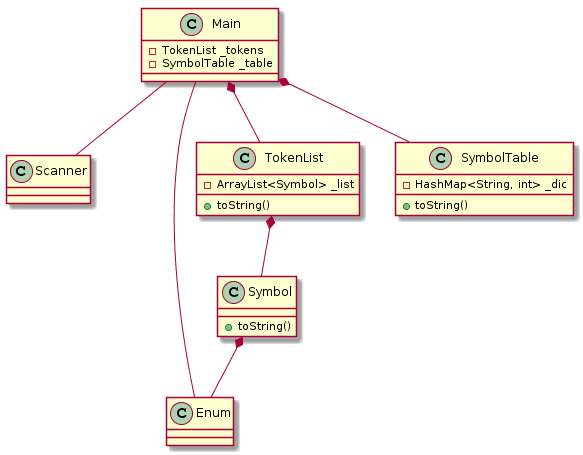
\includegraphics[scale=0.4]{./img/class_diag.png}\\
      \textit{Figure 2~-~Class model.}
    \end{center}
  
  \subsection{Regular expressions}
    pass
    
  \subsection{Tests}
    
    \lstinputlisting{../test/Search.imp}
    \lstinputlisting{../test/Sort.imp}

\section{How to set up the project}

\end{document}
